\section{Behavioral Pattern}
Ở phần Behavioral Patterns, ta có 10 mẫu Patterns cụ thể là \textbf{Chain of Responsibility}, \textbf{Command}, \textbf{Iterator}, \textbf{Mediator}, \textbf{Memento}, \textbf{Observer}, \textbf{State}, \textbf{Strategy}, \textbf{Template Method}, \textbf{Visitor}. Nhờ vào 10 mẫu này mà ta có các giải pháp để thực hiện hành vi của các đối tượng cũng như tương tác giữa các đối tượng với nhau để hoàn thành task được giao.\\
\subsection{Chain of Responsibility}
\subsubsection{Định nghĩa}
Chain of Responsibility là một mẫu thiết kế hành vi (behavioral design pattern) trong lập trình, nó cho phép một loạt các đối tượng xử lý một yêu cầu tuần tự. Yêu cầu được chuyển tiếp qua các đối tượng cho đến khi có một đối tượng trong chuỗi có thể xử lý yêu cầu đó hoặc khi không còn đối tượng nào có thể xử lý.
\subsubsection{Cách sử dụng}
Thông thương ở một số trường hợp sau ta hay sử dụng chain of responsibility:
\begin{itemize}
    \item Có nhiều hơn một đối tượng có khả thực xử lý một yêu cầu trong khi đối tượng cụ thể nào xử lý yêu cầu đó lại phụ thuộc vào ngữ cảnh sử dụng.
    \item Khi có nhiều đối tượng có thể xử lý một yêu cầu và bạn muốn cho phép các đối tượng này tự động chọn đối tượng xử lý thích hợp.
    \item Khi bạn muốn tạo ra một chuỗi linh hoạt và có thể thay đổi cấu trúc xử lý yêu cầu một cách động.
\end{itemize}
\subsubsection{Cấu trúc}
\begin{center}
    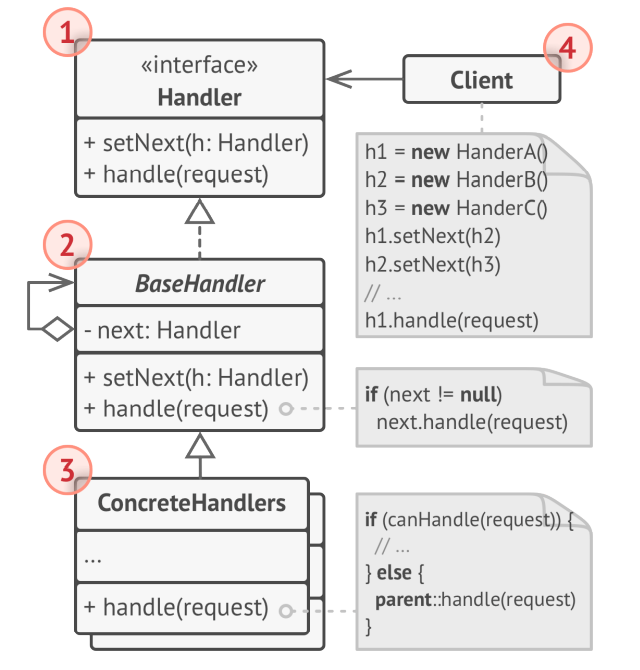
\includegraphics[scale= 0.45]{image/behavioral/cor.png}
\end{center}
\begin{itemize}
    \item Về cơ bản, cấu trúc này liên kết các class lại với nhau theo kiểu danh sách liên kết mỗi class này đều có hàm giải quyết vấn đề riêng của nó.
    \item Client sẽ sắp xếp thứ tự duyệt qua của các handlers.
\end{itemize}
Các thành phần chính:
\begin{itemize}
    \item Client là các dòng code ở trong main tạo ra các yêu cầu và yêu cầu đó sẽ được gửi đến các đối tượng tiếp nhận.
    \item Concrete Handler dùng để xử lí yêu cầu có con trỏ qua Concrete Handler khác nếu nó khong xử lí được.
    \item Handler là một interface hoặc abstract class có biến next.
    \item BaseHandler là một abstract class không bắt buộc có thể cài đặt các hàm chung cho chain of responsibility ở đây.
\end{itemize}
\subsubsection{Ưu điểm và Nhược điểm}
Ta có thể thấy tồn tại vài ưu nhược điểm sau
Ưu điểm:
\begin{itemize}
    \item Thay vì một đối tượng có khả năng xử lý yêu cầu chứa tham chiếu đến tất cả các đối tượng khác, nó chỉ cần một tham chiếu đến đối tượng tiếp theo. Tránh sự liên kết trực tiếp giữa đối tượng gửi yêu cầu (sender) và các đối tượng nhận yêu cầu (receivers).
    \item Dễ dàng thêm hoặc loại bỏ các bước xử lý trong chuỗi mà không ảnh hưởng đến các đối tượng khác.
\end{itemize}
Nhược điểm:
\begin{itemize}
    \item Một số yêu cầu có thể không được xử lý: Trường hợp tất cả Handler đều không xử lý
\end{itemize}
\subsubsection{Code Example}
\begin{itemize}
    \item Ta có một class Yêu cầu nâng cấp.
    \item Một loạt các class giải quyết yêu cầu nâng cấp có con trỏ chỉ đến bộ hanlder tiếp theo.
\end{itemize}
\begin{lstlisting}
#include <iostream>
#include <string>

class UpgradeRequest {
private:
    std::string component;
    std::string version;

public:
    UpgradeRequest(const std::string& component, const std::string& version)
        : component(component), version(version) {}

    std::string getComponent() const {
        return component;
    }

    std::string getVersion() const {
        return version;
    }
};

class UpgradeHandler {
protected:
    UpgradeHandler* nextHandler;

public:
    virtual void setNextHandler(UpgradeHandler* handler) {
        nextHandler = handler;
    }

    virtual void handleRequest(const UpgradeRequest& request) = 0;
};

class UIUpgradeHandler : public UpgradeHandler {
public:
    void handleRequest(const UpgradeRequest& request) override {
        if (request.getComponent() == "UI" && request.getVersion() == "2.0") {
            std::cout << "Upgrading UI component to version 2.0" << std::endl;
        } else if (nextHandler != nullptr) {
            nextHandler->handleRequest(request);
        } else {
            std::cout << "Upgrade request cannot be handled" << std::endl;
        }
    }
};

class DataUpgradeHandler : public UpgradeHandler {
public:
    void handleRequest(const UpgradeRequest& request) override {
        if (request.getComponent() == "Data" && request.getVersion() == "1.5") {
            std::cout << "Upgrading Data component to version 1.5" << std::endl;
        } else if (nextHandler != nullptr) {
            nextHandler->handleRequest(request);
        } else {
            std::cout << "Upgrade request cannot be handled" << std::endl;
        }
    }
};

class SecurityUpgradeHandler : public UpgradeHandler {
public:
    void handleRequest(const UpgradeRequest& request) override {
        if (request.getComponent() == "Security" && request.getVersion() == "3.2") {
            std::cout << "Upgrading Security component to version 3.2" << std::endl;
        } else if (nextHandler != nullptr) {
            nextHandler->handleRequest(request);
        } else {
            std::cout << "Upgrade request cannot be handled" << std::endl;
        }
    }
};

int main() {
    UpgradeHandler* uiUpgradeHandler = new UIUpgradeHandler();
    UpgradeHandler* dataUpgradeHandler = new DataUpgradeHandler();
    UpgradeHandler* securityUpgradeHandler = new SecurityUpgradeHandler();

    uiUpgradeHandler->setNextHandler(dataUpgradeHandler);
    dataUpgradeHandler->setNextHandler(securityUpgradeHandler);

    UpgradeRequest requestA("UI", "2.0");
    UpgradeRequest requestB("Data", "1.5");
    UpgradeRequest requestC("Security", "3.2");
    UpgradeRequest requestD("UI", "1.5");

    uiUpgradeHandler->handleRequest(requestA);
    uiUpgradeHandler->handleRequest(requestB);
    uiUpgradeHandler->handleRequest(requestC);
    uiUpgradeHandler->handleRequest(requestD);

    delete uiUpgradeHandler;
    delete dataUpgradeHandler;
    delete securityUpgradeHandler;

    return 0;
}

\end{lstlisting}
Ở hàm main, ta liên kết 3 hanlders lại với nhau. Ta có 4 yêu cầu từ khách hàng. Sau đó thực hiện giải quyết thì chỉ có duy nhất yêu cầu cuối cùng là không có bất cứ handler nào có thể giải quyết.\\
\newline
\textbf{Kết quả:}
\begin{lstlisting}
Upgrading UI component to version 2.0
Upgrading Data component to version 1.5
Upgrading Security component to version 3.2
Upgrade request cannot be handled
\end{lstlisting}
\subsubsection{Các Pattern liên quan}
\begin{itemize}
    \item Composite có thể được tích hợp chung. Ở trường hợp này các Leaf của CoR khi nhận yêu cầu sẽ được thực hiện tuần tự cho đến khi kết thúc.
    \item Có thể kết hợp với Command với các class Commands là các node lá của CoR và các command này sẽ được duyệt qua.
    \item Có thể kết hợp với Decorator bằng cách thêm thông tin vào các Leaf của CoR.
\end{itemize}

\subsection{Command}
\subsubsection{Định nghĩa}
Command là một mẫu thiết kế hành vi (behavioral design pattern) cho phép đóng gói các yêu cầu hoặc hành động vào một đối tượng riêng biệt. Nó chuyển đổi các yêu cầu thành một đối tượng độc lập, cho phép chúng ta thực hiện các yêu cầu, hàng loạt yêu cầu, hoặc hủy yêu cầu một cách linh hoạt.
\subsubsection{Cách sử dụng}
Thông thương, ta hay sử dụng mẫu thiết kế trên trong các trường hợp:
\begin{itemize}
    \item Khi bạn muốn tạo ra một hàng đợi các yêu cầu được thực thi theo thứ tự hoặc lưu trữ lịch sử các yêu cầu.
    \item Khi bạn muốn hỗ trợ hoạt động undo/redo.
    \item Phối hợp nhiều Command với nhau theo thứ tựtự.
\end{itemize}
\subsubsection{Cấu trúc}
\begin{center}
    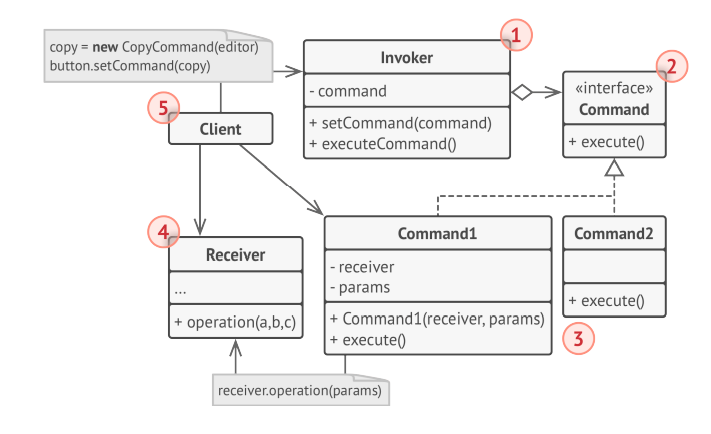
\includegraphics[scale= 0.6]{image/behavioral/command.png}
\end{center}
Các thành phần chính của mẫu:
\begin{itemize}
    \item Command là một interface hoặc abstract class chứa một phương thức thực thi, phương thức trừu tượng.
    \item ConcreteCommand là các subclass của Command định nghĩa operation.
    \item Invoker là một class tiếp nhận từ ConcreteCommand và gọi operation để thực thi.
    \item Receiver là một thành phần thực sử để xử lí cho case. Trong phương thức operation của ConcreteCommand chúng ta sẽ gọi method tương thích trong Receiver.
\end{itemize}
\subsubsection{Ưu điểm và Nhược điểm}
Có các ưu điểm và nhược điểm sau:
Ưu điểm:
\begin{itemize}
    \item Hỗ trợ các tính năng như undo/redo, quản lý lịch sử các yêu cầu.
    \item Giảm sự phụ thuộc giữa người gửi và người nhận yêu cầu.
\end{itemize}
Nhược điểm:
\begin{itemize}
    \item Có thể dẫn đến số lượng lớp lớn nếu có quá nhiều loại yêu cầu.
\end{itemize}

\subsubsection{Code Example}
\begin{itemize}
    \item Có một interface Command và 2 class LightOn và class LightOff được kế thừa.
    \item có class RemoteControl là Invoker có hàm excute để thực thi các lệnh.
\end{itemize}
\begin{lstlisting}
#include <iostream>
#include <string>
#include <vector>

// Command interface
class Command {
public:
    virtual void execute() = 0;
};

// Concrete command 1
class LightOnCommand : public Command {
private:
    std::string light;

public:
    LightOnCommand(const std::string& light) : light(light) {}

    void execute() override {
        std::cout << "Turn on " << light << " light" << std::endl;
    }
};

// Concrete command 2
class LightOffCommand : public Command {
private:
    std::string light;

public:
    LightOffCommand(const std::string& light) : light(light) {}

    void execute() override {
        std::cout << "Turn off " << light << " light" << std::endl;
    }
};

// Invoker
class RemoteControl {
private:
    std::vector<Command*> commands;

public:
    void setCommand(Command* command) {
        commands.push_back(command);
    }

    void executeCommands() {
        for (Command* command : commands) {
            command->execute();
        }
        commands.clear();
    }
};

int main() {
    // Create the invoker
    RemoteControl remote;

    // Create the commands
    Command* cmd1 = new LightOnCommand("Living Room");
    Command* cmd2 = new LightOnCommand("Bedroom");
    Command* cmd3 = new LightOffCommand("Bedroom");
    Command* cmd4 = new LightOffCommand("Living Room");

    // Set the commands
    remote.setCommand(cmd1);
    remote.setCommand(cmd2);
    remote.setCommand(cmd3);
    remote.setCommand(cmd4);

    // Execute the commands
    remote.executeCommands();

    // Clean up
    delete cmd1;
    delete cmd2;
    delete cmd3;
    delete cmd4;

    return 0;
}


\end{lstlisting}
Ở hàm main, ta tạo ra 4 lệnh, add nó vào remote rồi sau đó cho thực hiện cả 4 lệnh đó.\\
\newline
\textbf{Kết quả:}
\begin{lstlisting}
Turn on Living Room light
Turn on Bedroom light
Turn off Bedroom light
Turn off Living Room light
\end{lstlisting}
\subsubsection{Các Pattern liên quan}
\begin{itemize}
    \item CoR: nhận yêu cầu rôi thực hiện lần lượt các commands theo thứ tự.
    \item Mediator: thực hiện thông qua đối tượng gián tiếp.
    \item Observer: định nghĩa mối quan hệ một thay đổi các commands thay đổi theo.
\end{itemize}
\subsection{Iterator}
\subsubsection{Định nghĩa}
Iterator là một mẫu thiết kế hành vi (behavioral design pattern) cho phép truy cập tuần tự vào các phần tử của một tập hợp (collection) mà không tiết lộ cấu trúc nội bộ của nó. Nó cung cấp một cách tiếp cận thống nhất để duyệt qua các phần tử của một tập hợp mà không phụ thuộc vào kiểu cấu trúc dữ liệu của tập hợp đó.
\subsubsection{Cách sử dụng}
Ta sẽ sử dụng Pattern này trong các trường hợp:
\begin{itemize}
    \item Sử dụng mẫu Iterator khi collection của bạn có một cấu trúc dữ phức tạp, nhưng bạn muốn ẩn tính phức tạp chung của nó với các máy khác (để thuận tiện hoặc bảo mật).
    \item Khi được đặt trong logic kinh doanh của một ứng dụng, nó có thể làm lu mờ vai trò của source code gốc và làm cho nó khó bảo trì hơn. Với việc di chuyển source code đó đến các Iterator được chỉ định có thể giúp code của mình gọn gàng và sạch sẽ hơn.
    \item Sử dụng Iterator khi bạn muốn có một interface duy nhất để duyệt qua các phần tử của một tập hợp, code của mình có thể follow các cấu trúc dữ liệu khác nhau hoặc khi các loại cấu trúc chuỗi này chưa được biết trước.
\end{itemize}
\subsubsection{Cấu trúc}
\begin{center}
    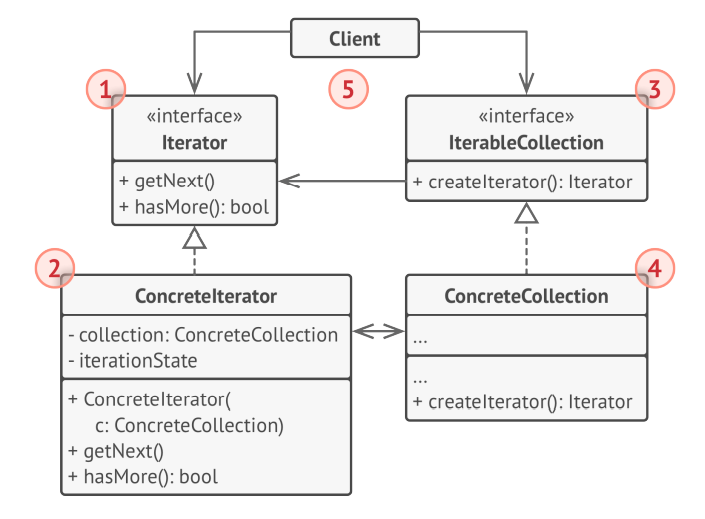
\includegraphics[scale= 0.6]{image/behavioral/iterator.png}
\end{center}
Các thành phần chính:
\begin{itemize}
    \item Một interface hay abstract class tên Iterator định nghĩa các hoạt động cần thiết.
    \item Concrete Iterator implement các phương thức trên.
    \item Collection Interface để khai báo một hoặc nhiều phương thức để nhận được các Iterator tương thích với collection.
    \item Concrete Collection trả về các phiên bản của một lớp Iterator cụ thể mỗi khi có các dòng code yêu cầu.
\end{itemize}
\subsubsection{Ưu điểm và Nhược điểm}
Có các ưu điểm và nhược điểm sau:
Ưu điểm:
\begin{itemize}
    \item Hỗ trợ nhiều cách duyệt qua các phần tử, bao gồm duyệt theo chiều thuận, chiều ngược và duyệt ngẫu nhiên.
    \item Chúng ta có thể truy cập song song trên cùng một tập hợp vì mỗi đối tượng iterator có chứa trạng thái riêng của nó.
\end{itemize}
Nhược điểm:
\begin{itemize}
    \item Sử dụng iterator có thể kém hiệu quả hơn so với việc duyệt qua các phần tử của bộ sưu tập một cách trực tiếp.
    \item Có thể không cần thiết nếu ứng dụng chỉ hoạt động với các collection đơn giản.
\end{itemize}
\subsubsection{Code Example}
\begin{itemize}
    \item Một interface Iterator và một VectorIterator là subclass.
\end{itemize}
\begin{lstlisting}
#include <iostream>
#include <vector>

// Iterator interface
class Iterator {
public:
    virtual bool hasNext() = 0;
    virtual int next() = 0;
};

// Concrete iterator
class VectorIterator : public Iterator {
private:
    std::vector<int>& vector;
    int index;

public:
    VectorIterator(std::vector<int>& vec) : vector(vec), index(0) {}

    bool hasNext() override {
        return index < vector.size();
    }

    int next() override {
        return vector[index++];
    }
};

// Client code
void printValues(Iterator& iterator) {
    while (iterator.hasNext()) {
        std::cout << iterator.next() << " ";
    }
    std::cout << std::endl;
}

int main() {
    std::vector<int> numbers = { 1, 2, 3, 4, 5 };
    VectorIterator iterator(numbers);

    printValues(iterator);

    return 0;
}

\end{lstlisting}
Ở hàm main, ta gọi một vector int là dùng iterator duyệt qua các giá trị đó.\\
\newline
\textbf{Kết quả:}
\begin{lstlisting}
1 2 3 4 5 
\end{lstlisting}
\subsubsection{Các Pattern liên quan}
\begin{itemize}
    \item Composite: ta thường dùng Iterator để duyệt qua cấu trúc cây.
    \item Memento: có thể kết hợp với Memento để lưu lại các trạng thái đã từng duyệt qua.
    \item Visitor: có thể kết hợp với Iterator để xem qua một cấu trúc dữ liệu phức tạp và thực hiện một số thao tác trên các phần tử của nó.
\end{itemize}

\subsection{Interpreter}
\subsubsection{Định nghĩa}
Interpreter là một mẫu Pattern thuộc Behavioral Pattern cung cấp giải pháp để tạo ra đối tượng dựa trên mô tả người dùng trong lúc hoạt động chương trình. Nó thực thi một dòng lệnh hoặc một khối lệnh một cách tuần tự tại thời điểm chạy chương trình. Interpreter thực thi các dòng lệnh bằng cách chuyển nó thành mã máy cho phép chạy ngay lặp tức.
\subsubsection{Cách sử dụng}
Thông thương, ta hay sử dụng mẫu thiết kế trên trong các trường hợp:
\begin{itemize}
    \item Cho phép lập trình viên phát triển và hiện thực mã lệnh nhanh mà không cần phải complie. Sau mỗi lần chỉnh sửa mã nguồn, lập trình viên có thể chạy và xem kết quả ngay lặp tức.
    \item  Interpreter thường được sử dụng cho các ngôn ngữ có cấu trúc chạy từ trên xuống dưới như Python, Javascript,...
\end{itemize}
\subsubsection{Cấu trúc}
\begin{center}
    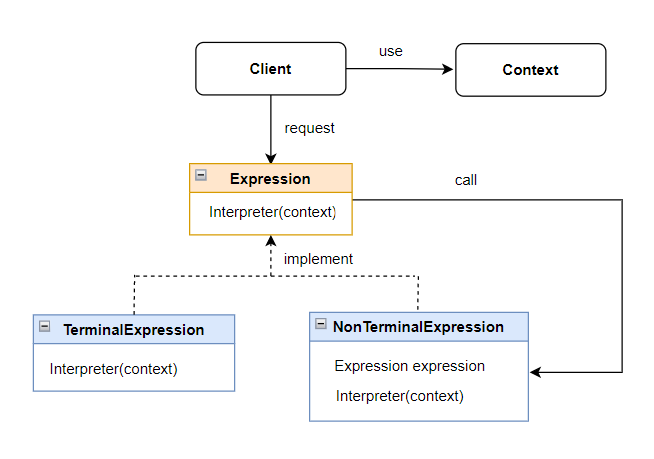
\includegraphics[scale= 0.6]{image/behavioral/interpreter.png}
\end{center}
Các thành phần chính của mẫu:
\begin{itemize}
    \item AbstractionExpression là một Class khai báo một giao diện cho việc thực thi một thao tác bất kì.
    \item TerminalExpression là một class cài đặt một thao tác thông dịch liên kết với những ký pháp đầu cuối, đóng vai trò một thể nghiệm được yêu cầu cho mọi ký pháp đầu cuối trong câu.
    \item NonterminalExpression là một class có thể chứa TerminalExpression bên trong và cũng có thể chứa một NonterminalExpression khác. Nó đóng vai trò như là “ngữ pháp” của ngôn ngữ đặc tả.
    \item Context: Là đối tượng thông tin để thực hiện thông dịch. Đối tượng này là toàn cục đối với quá trình thông dịch.
\end{itemize}
\subsubsection{Ưu điểm và Nhược điểm}
Có các ưu điểm và nhược điểm sau:
Ưu điểm:
\begin{itemize}
    \item Giảm số lượng những lớp con không cần thiết.
    \item Cho phép ẩn các chi tiết implement từ client.
    \item Vì không cần biên dịch trước, việc chỉnh sửa và chạy lại mã nguồn nhanh chóng.
    \item Interpreter có thể chạy trên nhiều nền tảng khác nhau mà không cần biên dịch lại.
\end{itemize}
Nhược điểm:
\begin{itemize}
    \item Interpreter phải dịch và thực thi từng dòng lệnh một tại thời điểm chạy, do đó tốn thời gian hơn so với việc biên dịch trước.
    \item Hiệu suất thấp.
    \item Đòi hỏi ngôn ngữ được xây dựng phải có cấu trúc đơn giản.
\end{itemize}

\subsubsection{Code Example}
\begin{itemize}
    \item Có một abtract class Expression để địng nghĩa dạng của kiểu lưu Expression.
    \item Các class Variable, Constant, Add, Subtract đại diện cho các biểu thức đại số (terminal và non-terminal) được kế thừa từ lớp Expresion ở trên.
\end{itemize}
\begin{lstlisting}
#include <iostream>
#include <string>
#include <unordered_map>

// Abstract Expression
class Expression {
public:
    virtual int interpret(std::unordered_map<char, int>& variables) = 0;
};

// Terminal Expression
class Variable : public Expression {
private:
    char variableName;
public:
    Variable(char name) : variableName(name) {}
    int interpret(std::unordered_map<char, int>& variables) override {
        return variables[variableName];
    }
};

// Terminal Expression
class Constant : public Expression {
private:
    int value;
public:
    Constant(int val) : value(val) {}
    int interpret(std::unordered_map<char, int>& variables) override {
        return value;
    }
};

// Non-terminal Expression
class Add : public Expression {
private:
    Expression* left;
    Expression* right;
public:
    Add(Expression* l, Expression* r) : left(l), right(r) {}
    int interpret(std::unordered_map<char, int>& variables) override {
        return left->interpret(variables) + right->interpret(variables);
    }
};

// Non-terminal Expression
class Subtract : public Expression {
private:
    Expression* left;
    Expression* right;
public:
    Subtract(Expression* l, Expression* r) : left(l), right(r) {}
    int interpret(std::unordered_map<char, int>& variables) override {
        return left->interpret(variables) - right->interpret(variables);
    }
};

// Client
int main() {
    std::unordered_map<char, int> variables;
    variables['x'] = 5;
    variables['y'] = 3;

    Expression* expression = new Subtract(
        new Add(new Variable('x'), new Variable('y')),
        new Constant(2)
    );

    int result = expression->interpret(variables);
    std::cout << "Result: " << result << std::endl;

    delete expression;

    return 0;
}


\end{lstlisting}
Trong phần main(), chúng ta khởi tạo các biến và xây dựng một biểu thức để tính toán (x + y - 2). Sau đó, chúng ta gọi hàm interpret() của biểu thức đó với một unorderedmap chứa giá trị của các biến (x = 5 và y = 3). Kết quả tính toán được in ra màn hình.
\\
\newline
\textbf{Kết quả:}
\begin{lstlisting}
Result: 6
\end{lstlisting}
\subsubsection{Các Pattern liên quan}
\begin{itemize}
    \item Composite là cây có trúc ngữ pháp trừu tượng
    \item Sử dụng Iterator để duyệt các dòng lệnh.
    \item Visitor có thể được sử dụng để duy trì hành vi trên mỗi nút trong cây cú pháp trừu tượng của lớp.
\end{itemize}
\subsection{Mediator}
\subsubsection{Định nghĩa}
Mediator là một mẫu thiết kế hành vi (behavioral design pattern) cho phép giảm sự phụ thuộc giữa các đối tượng và tạo một sự tương tác trung gian giữa chúng thông qua một đối tượng trung tâm được gọi là Mediator. Mediator đóng vai trò làm trung gian, điều phối và quản lý tất cả các tương tác giữa các đối tượng thành phần.
\subsubsection{Cách sử dụng}
Trong vài trường hợp sau, ta có thể áp dụng Pattern này vào:
\begin{itemize}
    \item Khi sự phụ thuộc giữa các đối tượng dẫn đến một hệ thống phức tạp và khó khăn trong việc bảo trì và mở rộng.
    \item Sử dụng khi tập hợp các đối tượng giao tiếp theo những cách thức được xác định rõ ràng nhưng cách thức đó quá phức tạp.
    \item Khi bạn muốn tạo một sự tương tác trung gian giữa các đối tượng mà không làm cho chúng gắn kết với nhau.
\end{itemize}
\subsubsection{Cấu trúc}
\begin{center}
    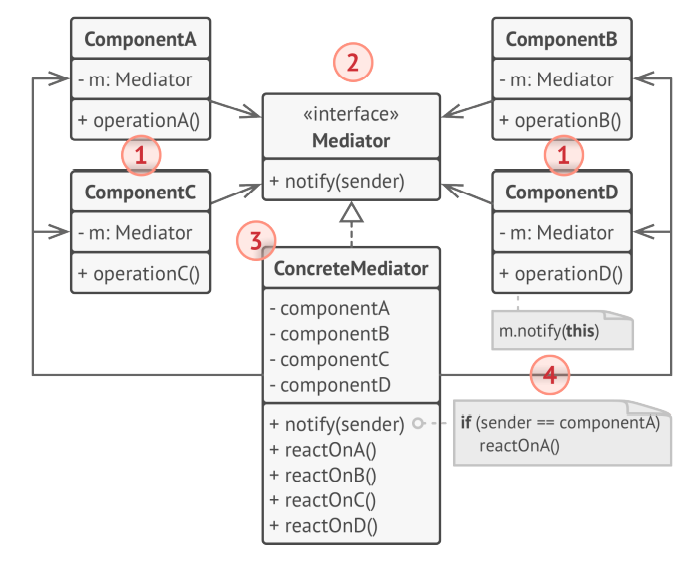
\includegraphics[scale=0.6]{image/behavioral/mediator.png}
\end{center}
\subsubsection{Ưu điểm và Nhược điểm}
Có các ưu điểm và nhược điểm sau:
Ưu điểm:
\begin{itemize}
    \item Đơn giản hóa cách giao tiếp giữa các đối tượng, Một Mediator sẽ thay thế mối quan hệ nhiều nhiều (many-to-many) giữa các component bằng quan hệ một-nhiều (one-to-many) giữa một mediator với các component.
    \item Quản lý tập trung, giúp làm rõ các component tương tác trong hệ thống như thế nào trong hệ thống.
    \item Giảm sự phụ thuộc giữa các đối tượng, làm cho hệ thống linh hoạt hơn và dễ dàng mở rộng.
    \item Tách biệt logic điều phối và logic của các đối tượng thành phần, làm cho mã dễ đọc và bảo trì hơn.
\end{itemize}
Nhược điểm:
\begin{itemize}
    \item Mediator có thể trở thành một điểm trung tâm phụ thuộc, làm giảm tính độc lập và sự tái sử dụng của các đối tượng thành phần.
\end{itemize}
\subsubsection{Code Example}
\begin{itemize}
    \item Có một interface Colleague và class User là subclass.
    \item Có một interface Mediator và class ChatRoom là subclass.
\end{itemize}
\begin{lstlisting}
#include <iostream>
#include <string>
#include <vector>

// Forward declaration
class Colleague;

// Mediator
class Mediator {
public:
    virtual void sendMessage(Colleague* sender, const std::string& message) = 0;
};

// Colleague (Abstract Base Class)
class Colleague {
protected:
    Mediator* mediator;

public:
    explicit Colleague(Mediator* mediator) : mediator(mediator) {}

    virtual void receiveMessage(const std::string& message) = 0;
    virtual void sendMessage(const std::string& message) = 0;
};

// Concrete Colleague
class User : public Colleague {
private:
    std::string name;

public:
    User(const std::string& name, Mediator* mediator) : name(name), Colleague(mediator) {}

    void receiveMessage(const std::string& message) override {
        std::cout << name << " received message: " << message << std::endl;
    }

    void sendMessage(const std::string& message) override {
        mediator->sendMessage(this, message);
    }
};

// Concrete Mediator
class ChatRoom : public Mediator {
private:
    std::vector<User*> users;

public:
    void addUser(User* user) {
        users.push_back(user);
    }

    void sendMessage(Colleague* sender, const std::string& message) override {
        for (auto user : users) {
            if (user != sender) {
                user->receiveMessage(message);
            }
        }
    }
};

int main() {
    ChatRoom chatRoom;

    User user1("Alice", &chatRoom);
    User user2("Bob", &chatRoom);
    User user3("Charlie", &chatRoom);

    chatRoom.addUser(&user1);
    chatRoom.addUser(&user2);
    chatRoom.addUser(&user3);

    user1.sendMessage("Hello, everyone!");
    user2.sendMessage("Hi, Alice!");

    return 0;
}

\end{lstlisting}
Ở hàm main, ta gọi 3 user cho vào chatRoom và thực hiện việc gửi tin nhắn.\\
\newline
\textbf{Kết quả:}
\begin{lstlisting}
Bob received message: Hello, everyone!
Charlie received message: Hello, everyone!
Alice received message: Hi, Alice!
Charlie received message: Hi, Alice!
\end{lstlisting}
\subsubsection{Các Pattern liên quan}
\begin{itemize}
    \item Chain of Responsibility truyền request lần lượt chứa các receiver tiềm năng cho đến khi có receiver thích hợp có thể giải quyết được. Command thì tạo ra các kết nối một chiều giữa các receiver và các sender.
    \item Mediator loại bỏ các kết nối trực tiếp giữa các receiver và các sender rồi bắt buộc chúng phải giao tiếp không trực tiếp thông qua đối tượng mediator.
    \item Observer cho phép các receiver chủ động trong việc subscribe và unsubscribe receiving requests.
    \item Facade thì định nghĩa một interface được đơn giản hóa đến các đối tượng của hệ thống con nhưng nó không tạo thêm các chức năng mới.
    \item Mediator thì sẽ trung gian hóa sự giao tiếp giữa các component trong hệ thống.
\end{itemize}
\subsection{Memento}
\subsubsection{Định nghĩa}
Memento là một mẫu thiết kế hành vi trong đó một đối tượng được tạo ra để lưu trữ trạng thái của một đối tượng khác và khôi phục lại trạng thái đó sau này mà không tiết lộ chi tiết cài đặt.
\subsubsection{Cách sử dụng}
Memento được sử dụng khi bạn muốn lưu trữ trạng thái của một đối tượng và khôi phục lại trạng thái đó sau này. Điều này có thể xảy ra trong các tình huống như:
\begin{itemize}
    \item Khi bạn muốn lưu trữ một checkpoint hoặc trạng thái tạm thời của một ứng dụng để có thể hoàn tác hoặc khôi phục lại trạng thái trước đó.
    \item Khi bạn muốn theo dõi và lưu lại lịch sử của một đối tượng để có thể quay lại các trạng thái trước đó.
\end{itemize}
\subsubsection{Cấu trúc}
\begin{center}
    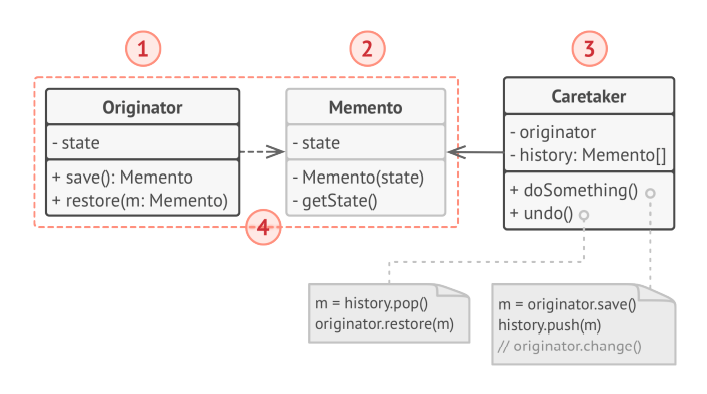
\includegraphics[scale = 0.6]{image/behavioral/memento.png}
\end{center}
\subsubsection{Ưu điểm và Nhược điểm}
Có các ưu điểm và nhược điểm sau:
Ưu điểm:
\begin{itemize}
    \item Nguyên tắc đơn trách nhiệm: Memento chỉ tương tác với nguồn gốc của nó và không gây phụ thuộc đối tượng khác.
    \item Bảo vệ dữ liệu: Dữ liệu bên trong Memento không thể truy cập hoặc sửa đổi từ bên ngoài.
    \item Khi có một số lượng lớn Memento được tạo ra có thể gặp vấn đề về bộ nhớ, performance của ứng dụng.
\end{itemize}
Nhược điểm:
\begin{itemize}
    \item Dùng quá nhiều bộ nhớ: Nếu Memento lưu trữ nhiều trạng thái hoặc đối tượng lớn, nó có thể tiêu tốn nhiều bộ nhớ.
    \item Hiệu suất: Nếu việc tạo và khôi phục Memento quá tốn kém và ảnh hưởng đến hiệu suất chung của ứng dụng.
\end{itemize}
\subsubsection{Code Example}
\begin{itemize}
    \item Có một class Memento chứa level và score.
    \item Một class Game có các phương thức và phải có hàm saveState để giữ trạng thái hiện tại.
    \item Class GameHistory lưu các memento của game.
\end{itemize}
\begin{lstlisting}
#include <iostream>
#include <vector>

// Memento: Represents the snapshot of the state
class Memento {
private:
    int level;
    int score;

public:
    Memento(int level, int score) : level(level), score(score) {}

    int getLevel() const {
        return level;
    }

    int getScore() const {
        return score;
    }
};

// Originator: Creates and restores from mementos
class Game {
private:
    int level;
    int score;

public:
    void playLevel(int level) {
        this->level = level;
        score = 0;
        std::cout << "Playing Level " << level << std::endl;
    }

    void increaseScore(int points) {
        score += points;
        std::cout << "Score increased by " << points << ". Current score: " << score << std::endl;
    }

    Memento saveState() const {
        return Memento(level, score);
    }

    void restoreState(const Memento& memento) {
        level = memento.getLevel();
        score = memento.getScore();
        std::cout << "Restored state: Level " << level << ", Score " << score << std::endl;
    }
};

// Caretaker: Manages the mementos
class GameHistory {
private:
    std::vector<Memento> mementos;

public:
    void addMemento(const Memento& memento) {
        mementos.push_back(memento);
    }

    Memento getMemento(int index) const {
        return mementos[index];
    }
};

int main() {
    Game game;
    GameHistory history;

    // Play Level 1
    game.playLevel(1);
    game.increaseScore(100);
    history.addMemento(game.saveState());

    // Play Level 2
    game.playLevel(2);
    game.increaseScore(150);
    history.addMemento(game.saveState());

    // Play Level 3
    game.playLevel(3);
    game.increaseScore(200);

    // Restore state from Level 2
    game.restoreState(history.getMemento(1));

    return 0;
}

\end{lstlisting}
Ở hàm main, ta thực hiện chơi 3 màn và restore lại màn 2.\\
\newline
\textbf{Kết quả:}
\begin{lstlisting}
Playing Level 1
Score increased by 100. Current score: 100
Playing Level 2
Score increased by 150. Current score: 150
Playing Level 3
Score increased by 200. Current score: 200
Restored state: Level 2, Score 150
\end{lstlisting}
\subsubsection{Các Pattern liên quan}
\begin{itemize}
    \item Két hợp với Command để thực hiện các lệnh hoàn tác.
    \item Kết hợp với Iterator để nắm bắt các trạng thái và thực hiên các lệnh khôi phục.
    \item Hoặc đơn giản chỉ cần ở thời điểm nào đó tạo Clone rồi thời điểm khác lại tạo Clone là ta đã có Memento bản thu nhỏ.
\end{itemize}
\subsection{Observer}
\subsubsection{Định nghĩa}
Observer là một mẫu thiết kế hành vi trong đó có một đối tượng chủ đạo (subject) duy trì danh sách các đối tượng quan sát (observers) và thông báo cho chúng về bất kỳ sự thay đổi nào trong trạng thái của nó. Điều này cho phép các đối tượng quan sát tự động cập nhật khi có sự thay đổi xảy ra.
\subsubsection{Cách sử dụng}
Ta sẽ sử dụng mẫu Pattern trên trong các trường hợp sau:
\begin{itemize}
    \item Sự thay đổi trạng thái ở 1 đối tượng cần được thông báo đến các đối tượng khác mà không phải giữ chúng liên kết quá chặt chẽ.
    \item Khi thay đổi một đối tượng yêu cầu việc thay đổi đến các đối tượng khác, và bạn không biết số lượng đối tượng cần thay đổi.
    \item Khi bạn muốn giảm sự phụ thuộc giữa các đối tượng và cho phép chúng hoạt động độc lập với nhau.
\end{itemize}
\subsubsection{Cấu trúc}
\begin{center}
    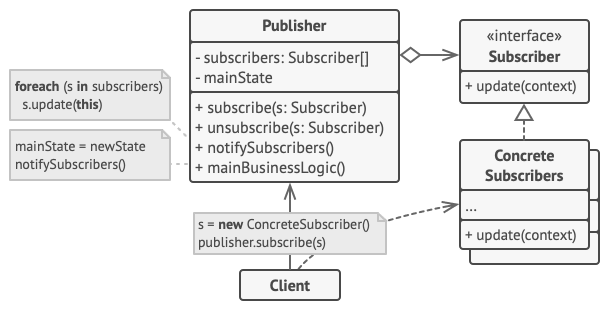
\includegraphics[scale= 0.6]{image/behavioral/observer.png}
\end{center}
\subsubsection{Ưu điểm và Nhược điểm}
Có các ưu điểm và nhược điểm sau:
Ưu điểm:
\begin{itemize}
    \item Sự thay đổi trạng thái ở 1 đối tượng có thể được thông báo đến các đối tượng khác mà không phải giữ chúng liên kết quá chặt chẽ.
    \item Không giới hạn số lượng Observer
    \item Đảm bảo sự tương tác giữa các đối tượng không phụ thuộc: Subject và observers không biết gì về sự tồn tại của nhau, do đó, chúng có thể hoạt động một cách độc lập và tái sử dụng được.
\end{itemize}
Nhược điểm:
\begin{itemize}
    \item Khi có nhiều observers và có nhiều thông báo được gửi đi, quá trình thông báo có thể gây ra sự chậm trễ và ảnh hưởng đến hiệu năng của hệ thống.
    \item Bởi vì các Observer không biết về sự hiện diện của nhau, nó có thể gây tốn nhiều chi phí của việc thay đổi Subject.
\end{itemize}
\subsubsection{Code Example}
\begin{itemize}
    \item Có interface Observer, Display là subclass có hàm update để cập nhật trạng thái.
    \item Có class WeatherStation.
\end{itemize}
\begin{lstlisting}
#include <iostream>
#include <vector>
#include <algorithm>

// Observer interface
class Observer {
public:
    virtual void update(int temperature) = 0;
};

// Subject class
class WeatherStation {
private:
    int temperature;
    std::vector<Observer*> observers;

public:
    void attach(Observer* observer) {
        observers.push_back(observer);
    }

    void detach(Observer* observer) {
        auto it = std::find(observers.begin(), observers.end(), observer);
        if (it != observers.end()) {
            observers.erase(it);
        }
    }

    void setTemperature(int newTemperature) {
        temperature = newTemperature;
        notify();
    }

    void notify() {
        for (auto observer : observers) {
            observer->update(temperature);
        }
    }
};

// Concrete Observer class
class Display : public Observer {
public:
    void update(int temperature) {
        std::cout << "Temperature changed: " << temperature << std::endl;
    }
};

int main() {
    // Create weather station and displays
    WeatherStation weatherStation;
    Display display1;
    Display display2;

    // Attach displays to the weather station
    weatherStation.attach(&display1);
    weatherStation.attach(&display2);

    // Set the temperature in the weather station
    weatherStation.setTemperature(25);

    // Detach one display from the weather station
    weatherStation.detach(&display1);

    // Set another temperature in the weather station
    weatherStation.setTemperature(30);

    // Attach display1 back to the weather station
    weatherStation.attach(&display1);

    // Set a third temperature in the weather station
    weatherStation.setTemperature(35);

    return 0;
}


\end{lstlisting}
Ở hàm main, ta tạo 2 display và lần lượt gán cho weatherStation đó với 2 loại Display. Sau đó, điều chỉnh nhiệt độ. Rồi bỏ đi một display trong weatherStation rồi lại điều chỉnh nhiệt độ. Xong lại thêm vào lại và điều chỉnh nhiệt đọ.\\
\newline
\textbf{Kết quả:}
\begin{lstlisting}
Temperature changed: 25
Temperature changed: 25
Temperature changed: 30
Temperature changed: 35
Temperature changed: 35
\end{lstlisting}
\subsubsection{Các Pattern liên quan}
\begin{itemize}
    \item Chain of Responsibility: duyệt theo thứ tự.
    \item Command: thiết kế mối quan hệ một chiều giữa người gửi và nhận.
    \item Mediator: dùng để loại bỏ kết nối trực tiếp giữa người gửi và nhận. 
    \item Observer: cho phép người nhận đăng kí động và hủy nhận yêu cầu.
\end{itemize}

\subsection{State}
\subsubsection{Định nghĩa}
State Pattern là một mẫu thiết kế thuộc nhóm Behavioral Pattern. State Pattern là một mẫu thiết kế hành vi cho phép một object thay đổi hành vi của nó khi trạng thái bên trong của nó thay đổi.
\subsubsection{Cách sử dụng}
Ta có thể sử dụng State Pattern trong các trường hợp sau:
\begin{itemize}
    \item Khi bạn có một object hoạt động khác nhau tùy thuộc vào trạng thái hiện tại của nó, số lượng trạng thái là rất lớn và code của trạng thái cụ thể thường xuyên thay đổi.
    \item Khi không muốn sử dụng nhiều câu lệnh điều kiện (if-else hoặc switch-case) để kiểm tra trạng thái của đối tượng.
    \item Khi bạn có nhiều code trùng lặp qua các trạng thái và chuyển đổi tương tự của State Pattern dựa trên điều kiện.
\end{itemize}
\subsubsection{Cấu trúc}
\begin{center}
    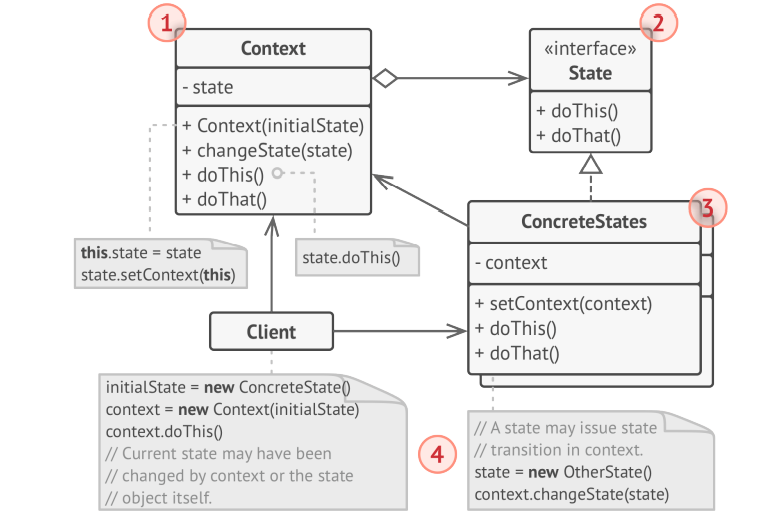
\includegraphics[scale=0.6]{image/behavioral/state.png}
\end{center}
\subsubsection{Ưu điểm và Nhược điểm}
Ta có rất nhiều ưu nhược điểm như sau:\\\\
Ưu điểm:
\begin{itemize}
    \item Mẫu State cho phép mô hình hóa trực quan các trạng thái khác nhau và cách chúng tương tác với nhau.
    \item Thay vì sử dụng nhiều câu lệnh điều kiện, mẫu State giúp tách biệt logic của từng trạng thái thành các lớp riêng biệt, giảm sự phức tạp của mã.
\end{itemize}
Nhược điểm:
\begin{itemize}
    \item Mẫu State có thể tạo ra nhiều lớp con để đại diện cho từng trạng thái, dẫn đến việc tăng số lượng lớp trong mã nguồn.
    \item Logic của mỗi trạng thái có thể phân mảnh trong các lớp con khác nhau, làm cho mã nguồn khó hiểu và duy trì.
\end{itemize}
\subsubsection{Code Example}
\begin{itemize}
    \item Có các class State con.
    \item Một các Context chữa State hiện tại.
\end{itemize}
\begin{lstlisting}
#include <iostream>

// State interface
class State {
public:
    virtual void handleState() = 0;
};

// Concrete states
class ConcreteStateA : public State {
public:
    void handleState() override {
        std::cout << "Handling state A." << std::endl;
    }
};

class ConcreteStateB : public State {
public:
    void handleState() override {
        std::cout << "Handling state B." << std::endl;
    }
};

// Context class
class Context {
private:
    State* currentState;

public:
    Context() {
        currentState = nullptr;
    }

    void setState(State* state) {
        currentState = state;
    }

    void request() {
        if (currentState) {
            currentState->handleState();
        }
    }
};

int main() {
    Context context;

    // Set initial state to A
    ConcreteStateA stateA;
    context.setState(&stateA);
    context.request();

    // Change state to B
    ConcreteStateB stateB;
    context.setState(&stateB);
    context.request();

    return 0;
}

\end{lstlisting}
Ở hàm main, Ta tạo 2 state r set State cho context r request nó sau đó chuyển context qua state khác rồi request nó.\\
\newline
\textbf{Kết quả:}
\begin{lstlisting}
Handling state A.
Handling state B.
\end{lstlisting}
\subsubsection{Các Pattern liên quan}
\begin{itemize}
    \item Bridge, State, Strategy có cấu trúc rất giống nhau. Tuy nhiên, chúng đều giải quyết các vấn đề khác nhau.
    \item State là bản mở rộng của Strategy. Cả hai Pattern đều dựa trên thành phần: chúng thay đổi hành vi của ngữ cảnh bằng cách ủy quyền một số công việc cho các object trợ giúp.
    \item Gần giống strategy, chuyển đổi các chiến lược thông qua các phương thức được định nghĩa trong interface. State không hạn chế sự phụ thuộc giữa các trạng thái cụ thể, cho phép chúng thay đổi trạng thái của ngữ cảnh theo ý muốn.
\end{itemize}



\subsection{Strategy}
\subsubsection{Định nghĩa}
Strategy (Chiến lược) là một mẫu thiết kế hành vi cho phép đối tượng thay đổi thuật toán được sử dụng trong quá trình thực thi một hành động cụ thể mà không ảnh hưởng đến các đối tượng khác hoặc cấu trúc của chúng. Mẫu này tách rời thuật toán khỏi đối tượng sử dụng nó, giúp tăng tính linh hoạt và tái sử dụng trong việc áp dụng các thuật toán khác nhau.
\subsubsection{Cách sử dụng}
Ta có thể sử dụng Strategy Pattern trong các trường hợp sau:
\begin{itemize}
    \item Khi có một hành động cần thực hiện, nhưng có nhiều thuật toán khác nhau có thể được áp dụng, và cần linh hoạt trong việc chọn thuật toán tại thời điểm chạy.
    \item Khi muốn tránh sự phức tạp của việc sử dụng nhiều câu lệnh điều kiện (if-else hoặc switch-case) để chọn thuật toán.
    \item Khi muốn tránh sự phức tạp của việc sử dụng nhiều câu lệnh điều kiện (if-else hoặc switch-case) để chọn thuật toán.
\end{itemize}
\subsubsection{Cấu trúc}
\begin{center}
    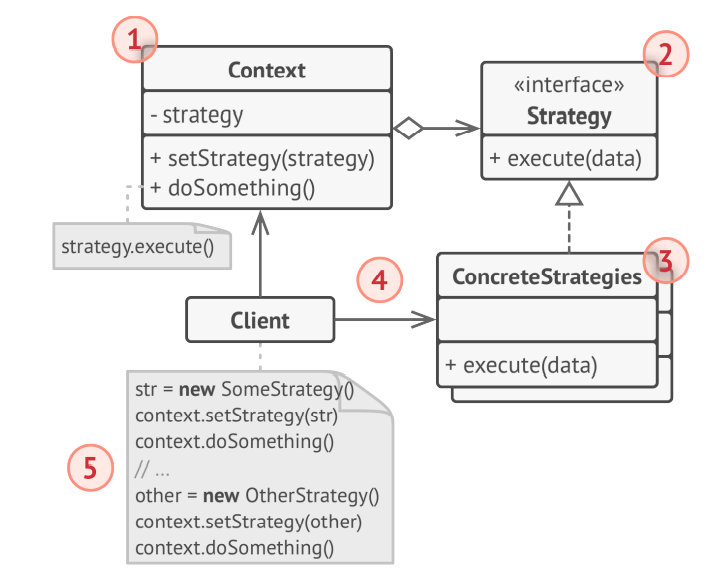
\includegraphics[scale=0.6]{image/behavioral/strategy.png}
\end{center}
\subsubsection{Ưu điểm và Nhược điểm}
Ta có rất nhiều ưu nhược điểm như sau:\\\\
Ưu điểm:
\begin{itemize}
    \item Linh hoạt và dễ dàng thay đổi thuật toán tại thời điểm chạy.
    \item Khi thay đổi thuật toán hoặc khi thêm mới thuật toán, không cần thay đổi code phần context.
    \item Có thể thay thế việc kế thừa bằng việc encapsulate thuật toán.
\end{itemize}
Nhược điểm:
\begin{itemize}
    \item Tăng số lượng các lớp và đối tượng, đặc biệt khi có nhiều thuật toán khác nhau.
    \item Cần phải hiểu rõ các thuật toán khác nhau để chọn và sử dụng một cách phù hợp.
\end{itemize}
\subsubsection{Code Example}
\begin{itemize}
    \item Có một interface và 2 concrete class thực hiện hóa 2 hàm sort.
    \item Một class Sorter có Strategy sort trong đó.
\end{itemize}
\begin{lstlisting}
#include <iostream>

// Strategy interface
class SortingStrategy {
public:
    virtual void sort(int* arr, int size) = 0;
};

// Concrete strategies
class QuickSortStrategy : public SortingStrategy {
public:
    void sort(int* arr, int size) override {
        std::cout << "Sorting using Quick Sort." << std::endl;
        // Perform Quick Sort algorithm
    }
};

class MergeSortStrategy : public SortingStrategy {
public:
    void sort(int* arr, int size) override {
        std::cout << "Sorting using Merge Sort." << std::endl;
        // Perform Merge Sort algorithm
    }
};

// Context class
class Sorter {
private:
    SortingStrategy* strategy;

public:
    void setStrategy(SortingStrategy* sortingStrategy) {
        strategy = sortingStrategy;
    }

    void sortArray(int* arr, int size) {
        strategy->sort(arr, size);
    }
};

int main() {
    int arr[] = {5, 2, 8, 1, 9};
    int size = sizeof(arr) / sizeof(arr[0]);

    Sorter sorter;

    QuickSortStrategy quickSortStrategy;
    MergeSortStrategy mergeSortStrategy;

    sorter.setStrategy(&quickSortStrategy);
    sorter.sortArray(arr, size);

    sorter.setStrategy(&mergeSortStrategy);
    sorter.sortArray(arr, size);

    return 0;
}

\end{lstlisting}
Ở hàm main, ta tạo ra 2 kiểu sort rồi thực hiện tuần tự 2 loại sort.\\
\newline
\textbf{Kết quả:}
\begin{lstlisting}
Sorting using Quick Sort.
Sorting using Merge Sort.
\end{lstlisting}
\subsubsection{Các Pattern liên quan}
\begin{itemize}
    \item Bridge có cấu trúc gống Strategy dựa trên composition.
    \item Command: giống nhau ở chỗ tham số hóa một đối tượng và hành động.
    \item State: là một bản mở rộng của Strategy.
\end{itemize}
\subsection{Template Method}
\subsubsection{Định nghĩa}
Template Method (Phương pháp mẫu) là một mẫu thiết kế hành vi cho phép định nghĩa một bản thiết kế mẫu cho một thuật toán và để các bước cụ thể của thuật toán được triển khai bởi các lớp con. Mẫu này xác định một khung (template) cho quy trình thực hiện một nhiệm vụ, trong đó một số bước được định nghĩa trong lớp gốc và các bước khác được chuyển giao cho các lớp con để triển khai.
\subsubsection{Cách sử dụng}
Ta có thể sử dụng Template Method Pattern trong các trường hợp sau:
\begin{itemize}
    \item Khi có một thuật toán với nhiều bước và mong muốn cho phép tùy chỉnh chúng trong lớp con.
    \item Mong muốn chỉ có một triển khai phương thức trừu tượng duy nhất của một thuật toán.
    \item Khi có một thuật toán chung, nhưng các bước cụ thể của thuật toán có thể thay đổi hoặc mở rộng bởi các lớp con.
    \item Khi muốn tránh việc lặp lại mã trong các lớp con bằng cách di chuyển các bước chung vào lớp gốc.
\end{itemize}
\subsubsection{Cấu trúc}
\begin{center}
    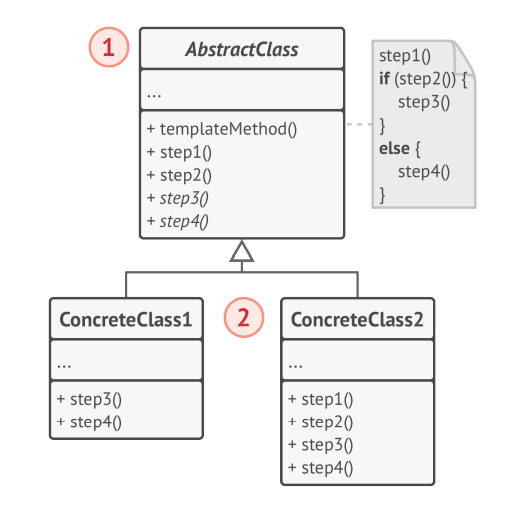
\includegraphics[scale=0.6]{image/behavioral/template.png}
\end{center}
\subsubsection{Ưu điểm và Nhược điểm}
Ta có rất nhiều ưu nhược điểm như sau:\\\\
Ưu điểm:
\begin{itemize}
    \item Các lớp con có thể thay đổi hoặc mở rộng các bước cụ thể của thuật toán mà không ảnh hưởng đến cấu trúc chung.
    \item  Mỗi bước của thuật toán được triển khai trong một phương thức riêng biệt, giúp tách rời và quản lý từng bước một.
    \item Cho phép người dùng override chỉ một số phần nhất định của thuật toán lớn, làm cho chúng ít bị ảnh hưởng hơn bởi những thay đổi xảy ra với các phần khác của thuật toán.
\end{itemize}
Nhược điểm:
\begin{itemize}
    \item Template method có càng nhiều bước để override càng khó bảo trì.
    \item Cần hiểu rõ khung (template) và cách các bước cụ thể được triển khai trong các lớp con.
\end{itemize}
\subsubsection{Code Example}
\begin{lstlisting}
#include <iostream>

// Abstract class defining the template method
class AbstractClass {
public:
    // Template method defining the algorithm
    void templateMethod() {
        step1();
        step2();
        step3();
    }

protected:
    virtual void step1() = 0;
    virtual void step2() = 0;
    virtual void step3() = 0;
};

// Concrete class implementing the template method
class ConcreteClass : public AbstractClass {
protected:
    void step1() override {
        std::cout << "ConcreteClass: Step 1" << std::endl;
    }

    void step2() override {
        std::cout << "ConcreteClass: Step 2" << std::endl;
    }

    void step3() override {
        std::cout << "ConcreteClass: Step 3" << std::endl;
    }
};

int main() {
    AbstractClass* abstractClass = new ConcreteClass();
    abstractClass->templateMethod();

    delete abstractClass;

    return 0;
}

\end{lstlisting}
Kết quả:
\begin{lstlisting}
ConcreteClass: Step 1
ConcreteClass: Step 2
ConcreteClass: Step 3
\end{lstlisting}
\subsubsection{Các Pattern liên quan}
\begin{itemize}
    \item Factory Method có thể đóng vai trò như một bước trong Template method là cơ sở chuyên môn hóa của Template Method.
\end{itemize}
\subsection{Visitor}
\subsubsection{Định nghĩa}
Visitor (Người ghé thăm) là một mẫu thiết kế hành vi cho phép thực hiện các thao tác trên các đối tượng của một tập hợp các lớp khác nhau mà không làm thay đổi cấu trúc của chúng. Mẫu này cho phép bạn định nghĩa các thao tác mới mà không phải thay đổi các lớp đã tồn tại và tách rời logic của các thao tác khỏi cấu trúc của các đối tượng.
\subsubsection{Cách sử dụng}
Ta có thể sử dụng Visitor Pattern trong các trường hợp sau:
\begin{itemize}
    \item Sử dụng khi cần thực hiện thao tác trên tất cả các phần tử của cấu trúc đối tượng phức tạp.
    \item Sử dụng khi một hành vi chỉ có ý nghĩa trong một số lớp của hệ thống phân cấp lớp, nhưng không có ý nghĩa trong các lớp khác.
    \item Khi có nhiều thao tác khác nhau cần thực hiện trên các đối tượng, và không muốn thay đổi các lớp của chúng.
\end{itemize}
\subsubsection{Cấu trúc}
\begin{center}
    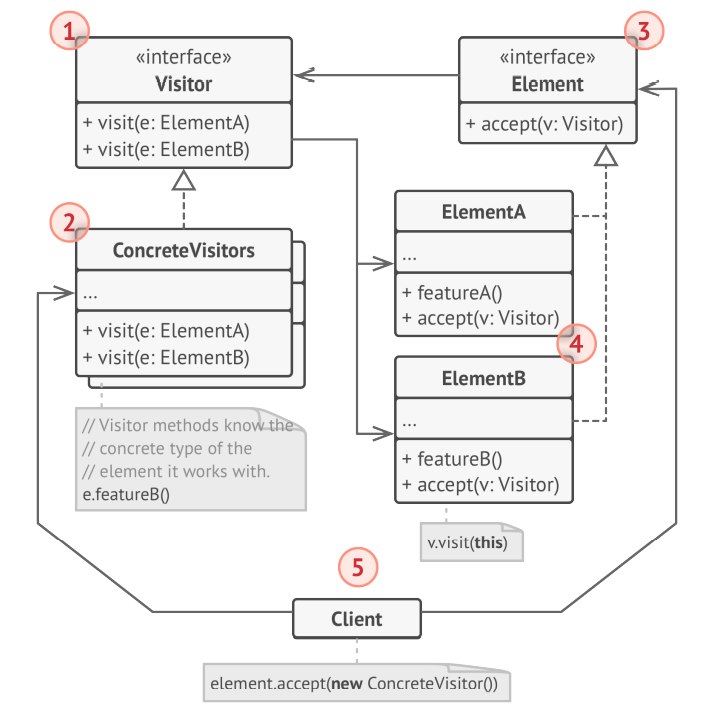
\includegraphics[scale=0.6]{image/behavioral/visitor.png}
\end{center}
\subsubsection{Ưu điểm và Nhược điểm}
Ta có rất nhiều ưu nhược điểm như sau:\\\\
Ưu điểm:
\begin{itemize}
    \item Một đối tượng visitor có thể tích lũy một số thông tin hữu ích khi làm việc với nhiều đối tượng khác nhau. Điều này có thể giúp ích khi ta muốn duyệt qua một số cấu trúc đối tượng phức tạp, chẳng hạn như cây đối tượng và áp dụng visitor cho từng đối tượng của cấu trúc này.
    \item Visitor cho phép tách rời logic của các thao tác khỏi cấu trúc của các đối tượng, giúp duy trì nguyên tắc đơn trách nhiệm (single responsibility principle).
    \item Visitor cho phép bạn thực hiện các thao tác khác nhau trên các đối tượng mà không cần thay đổi cấu trúc của chúng.
\end{itemize}
Nhược điểm:
\begin{itemize}
    \item Mẫu Visitor có thể làm tăng sự phức tạp của mã, đặc biệt khi có nhiều lớp và các thao tác phức tạp.
    \item Cần cập nhật tất cả visitor mỗi khi một lớp được thêm vào hoặc xóa khỏi hệ thống phân cấp phần tử.
    \item Các visitor có thể thiếu quyền truy cập cần thiết vào các trường riêng tư và phương thức của các phần tử mà họ phải làm việc với.
    \item Truyền đối tượng Visitor đến các đối tượng được ghé thăm có thể ảnh hưởng đến hiệu suất, đặc biệt khi có nhiều lớp và thao tác phức tạp.
\end{itemize}
\subsubsection{Code Example}
\begin{itemize}
    \item Có interface Element và 2 subclass.
    \item Có Abstract class Visitor và ConcreteVisitor.
\end{itemize}
\begin{lstlisting}
#include <iostream>
#include <vector>

// Forward declaration of classes
class ConcreteElementA;
class ConcreteElementB;

// Abstract Visitor class
class Visitor {
public:
    virtual void visit(ConcreteElementA* element) = 0;
    virtual void visit(ConcreteElementB* element) = 0;
};

// Abstract Element class
class Element {
public:
    virtual void accept(Visitor* visitor) = 0;
};

// Concrete Element A
class ConcreteElementA : public Element {
public:
    void accept(Visitor* visitor) override {
        visitor->visit(this);
    }

    std::string operationA() {
        return "ConcreteElementA";
    }
};

// Concrete Element B
class ConcreteElementB : public Element {
public:
    void accept(Visitor* visitor) override {
        visitor->visit(this);
    }

    std::string operationB() {
        return "ConcreteElementB";
    }
};

// Concrete Visitor
class ConcreteVisitor : public Visitor {
public:
    void visit(ConcreteElementA* element) override {
        std::cout << "ConcreteVisitor: Visit " << element->operationA() << std::endl;
    }

    void visit(ConcreteElementB* element) override {
        std::cout << "ConcreteVisitor: Visit " << element->operationB() << std::endl;
    }
};

int main() {
    // Create elements
    ConcreteElementA elementA;
    ConcreteElementB elementB;

    // Create visitor
    ConcreteVisitor visitor;

    // Accept visitor on elements
    elementA.accept(&visitor);
    elementB.accept(&visitor);

    return 0;
}

\end{lstlisting}
Ở hàm main, tạo ra 2 elements và một visitor cơ bản. Sau đó ta cho 2 elements này chấp nhận Visitor và cho ra kết quả.\\
\newline
\textbf{Kết quả:}
\begin{lstlisting}
ConcreteVisitor: Visit ConcreteElementA
ConcreteVisitor: Visit ConcreteElementB
\end{lstlisting}
\subsubsection{Các Pattern liên quan}
\begin{itemize}
    \item Một phiên bản hiệu quả của Command.
    \item Dùng Visitor để thực hiện thao tác trên cây Composite.
    \item Kết hợp với Iterator để duyệt qua cấu trúc dữ liệu phức tạp và thực hiện một vài Operation trên các phần tử của nó.
\end{itemize}